\section{Lightning Network overview}
\label{sec:ov-ln}

  \noindent {\bf Two-party channels.}
    The aim of LN is to enable fast, cheap, off-chain transactions,
    without compromising security. Specifically no trust between counterparties
    is needed. This is achieved as follows: Two parties that plan to have
    recurring monetary exchanges lock up some funds with one special on-chain
    transaction. We say that they opened a new channel. They can then transact
    with the locked funds multiple times solely by interacting privately,
    without informing the blockchain. If they want to use their funds in the
    usual, on-chain way again, they have to close the channel and unlock the
    funds with one more on-chain transaction. Each party can unilaterally close
    the channel and retrieve the coins they are entitled to -- according to the
    latest channel state -- and thus neither party has to trust the other.

    In more detail, to open a channel \alice{} and \bob{} first exchange
    a number of keys and desired timelocks $\mathrm{relDel}_A,
    \mathrm{relDel}_B$ (explained below) and then build locally some
    transactions. The ``funding transaction'' $F$ contains a 2-of-2 multisig
    output with one ``funding'' public key $pk_{F, A}, pk_{F, B}$ for each
    counterparty. This multisig output needs signatures for both
    designated public keys in order to be spent. $F$ is funded with
    $c_F$ coins that belong only to one of the two parties, say \alice.

    \begin{figure}[H]
    \centering
    \begin{pspicture}
      \drawtx{funding}{
        {{},{}}%
      }{
        {{$pk_{F{,} A} \wedge pk_{F{,} B}$},{$c_F$}}%
      }
    \end{pspicture}
    \label{fig:ln:funding}
    \caption{Funding TX (on-chain): Rules over, coins below output.}
    \end{figure}

    Each party also builds a slightly different version of the ``commitment
    transaction'' $C_A, C_B$. \alice{} uses her ``delayed payment'' key
    $pk_{\mathrm{dcom}, A}$ and \bob's ``revocation'' key $pk_{\mathrm{rev}, B}$
    (received before), whereas \bob{} uses \alice's ``payment'' key
    $pk_{\mathrm{com}, A}$ (received before). Both $C_A$ and $C_B$ spend the
    funding output of $F$ and allow \alice{} to retrieve her funds if she acts
    honestly, as we will explain shortly. \alice{} sends \bob{} the signature of
    $C_B$ made with her $sk_{F, A}$ and vice-versa.

    \begin{figure}[H]
    \centering
    \begin{pspicture}
      \drawtx{$\mathrm{comm}_A$}{
        {{$\sigma_{F{,} A} \wedge \sigma_{F{,} B}$},{funding}}%
      }{
        {{$pk_{\mathrm{rev}{,} B} \vee$,
        $(\mathrm{relDel}_B \wedge pk_{\mathrm{dcom}{,} A})$},{$c_F$}}%
      }
    \end{pspicture}
    \label{fig:ln:commitment:alice}
    \caption{\alice's initial commitment TX (off-chain): Required data over
    input, spent output below input.}
    \end{figure}

    \begin{figure}[H]
    \centering
    \begin{pspicture}
      \drawtx{$\mathrm{comm}_B$}{
        {{$\sigma_{F{,} A} \wedge \sigma_{F{,} B}$},{funding}}%
      }{
        {{$pk_{\mathrm{com}{,} A}$},{$c_F$}}%
      }
    \end{pspicture}
    \label{fig:ln:commitment:bob}
    \caption{\bob's initial commitment TX (off-chain): All coins belong to
    \alice, so she can immediately spend them if \bob{} closes.}
    \end{figure}

    \begin{figure*}
      % using png from GIMP. TODO: build tx composer and use that instead
      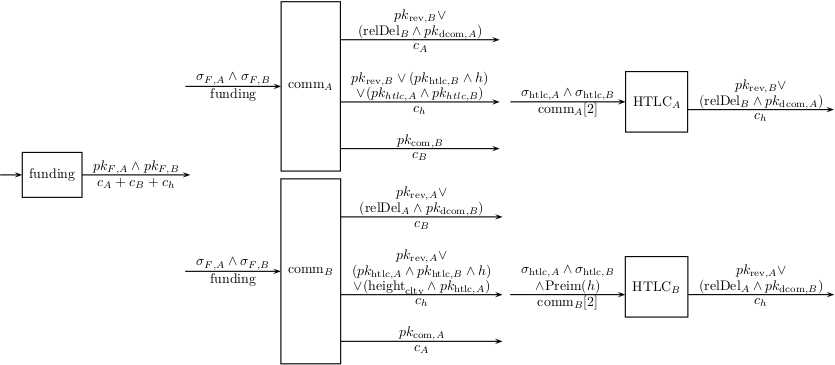
\includegraphics[width=\textwidth]{all-txs-figure}
      \caption{All transactions of an open channel with an HTLC in
      flight. \alice{} owns $c_A$ coins, \bob{} $c_B$ coins, and $c_h$ coins
      will be transferred to \bob{} if he discloses the preimage of $h$ until
      the ledger has $\mathrm{height}_{\mathrm{cltv}}$ blocks, otherwise they
      will return to \alice. ``funding'' is in the ledger, \alice{} keeps
      locally ``$\mathrm{comm}_A$'' and ``$\mathrm{HTLC}_A$'', and \bob{} keeps
      ``$\mathrm{comm}_B$'' and ``$\mathrm{HTLC}_B$''.}
      \label{fig:all-txs}
    \end{figure*}

    She now broadcasts $F$; once both parties see that it is confirmed,
    they generate and exchange new ``commitment'' keys (used for
    updating the channel later) and the channel is open.

    Every time they want to make a payment to each other, they exchange a series
    of messages that have two effects. First, a new pair of commitment
    transactions, along with their signatures by the funding keys, is created,
    one for each counterparty. Each of these transactions ensures that, if
    broadcast, each party will be able to spend the appropriate share from the
    coins contained in the funding output. Second, the two old commitment
    transactions are revoked. This ensures that no party can close a channel
    using an old commitment transaction which may be more beneficial to her than
    the latest one.

    Invalidating past commitments requires some care. The reason is that it is
    impossible to actually make past commitments invalid without spending the
    funding output on-chain; doing this for every update would however
    defeat the purpose of LN. The following idea is leveraged instead: If
    \alice{} broadcasts an old commitment and \bob{} sees it, he can punish
    \alice{} by taking all the money in the channel. Therefore \alice{} is
    technically able to broadcast an old commitment, but has no financial
    benefit in doing so. The same reasoning holds if \bob{} broadcasts
    an old commitment. On the donwside this imposes the requirement that
    parties must observe the blockchain periodically --- see below the
    explanation of timelocks and how they facilitate a time window within which
    parties should react.

    The punishing mechanism operates as follows. Suppose \alice{} considers
    posting her old local commitment which has an output that carries her old
    share of the funds. This output can be spent in two ways: either with a
    signature by \alice's ``delayed payment'' secret key
    $sk_{\mathrm{dcom}, A}$ which is a usual ECDSA key, or with a
    signature by \bob's ``revocation'' secret key $sk_{\mathrm{rev},
    B}$, which is also an ECDSA key, but with an additional characteristic that
    we will explain soon. Thus, if \alice{} broadcasts an old commitment, \bob{}
    will be able to obtain her funds by spending her output using his
    ``revocation'' key. This privilege of course opens the possibility for
    \bob{} to abuse it (in particular, when a channel is closed --- see below
    --- \bob{} may steal \alice's funds by using such a revocation key) and
    hence this side effect should also be carefully mitigated. The mitigation
    has the following form. At the time of creation of a new commitment, both
    parties will know \bob's ``revocation'' public key $pk_{\mathrm{rev}, B}$,
    but no party knows its corresponding secret -- the key can only be computed
    by combining one secret value $sk_{\mathrm{com}, n, A}$ that
    \alice{} knows and one secret value $sk_{\mathrm{com}, n, B}$ that
    \bob{} knows. \alice{} therefore can prevent \bob{} from using his
    revocation key until she sends him $sk_{\mathrm{com}, n, A}$.
    Therefore, \alice{} will send \bob{} $sk_{\mathrm{com}, n, A}$ only
    after the new commitment transaction is built and signed. Thus \bob{} cannot
    abuse his revocation key on a commitment before this transaction is revoked.
    We note that the underlying cryptographic mechanism  that enables such
    ``revocation keys'' is not straightforward and, as part of our
    contributions, we formalise it as a new two-party cryptographic primitive.
    We call it ``combined signature'' and we prove that the construction hidden
    in the LN implementation realizes it in the random oracle model under the
    assumption that the underlying digital signature scheme is secure in
    Appendix~\ref{appendix:combinedsign}.

    The last element needed to make channel updates secure is the
    already mentioned ``relative timelock''. If \alice{} broadcasts a
    commitment transaction, she is not allowed to immediately spend her funds
    with her ``delayed payment'' key. Instead, she has to wait for the
    transaction to reach a pre-agreed block depth (the relative timelock,
    negotiated during the opening of the channel and hardcoded in the
    output script of the commitment transaction) in order to give some time to
    \bob{} to see the transaction and, if it does not correspond to the latest
    version of the channel, punish her with his ``revocation'' key. This avoids
    a scenario in which \alice{} broadcasts an old commitment transaction and
    immediately spends her output, which would prevent \bob{} from ever proving
    that this commitment was old.

    Lastly, if \alice{} wants to unilaterally close a channel, all she has to do
    is broadcast her latest local commitment (the only one not revoked)
    and any outstanding HTLC transactions (explained below) and wait
    for the timelock to expire in order to spend her funds. The LN specification
    further allows for cooperative channel closure, achieved by negotiating and
    broadcasting the ``closing transaction'' which is not encumbered
    with a timelock, providing immediate availability of funds.

    As mentioned timelocks provide specific time windows within which both
    parties have to check the blockchain in order to punish a misbehaving
    counterparty who  broadcasts an old commitment transaction. This means that
    parties have to be regularly online to safeguard against theft.
    Furthermore, LN makes it possible to trustlessly outsource this to
    so-called watchtowers, but this mechanism is not analyzed in the current
    work.

  \noindent {\bf Multi-hop payments.}
    Having funds locked down for exclusive use with a particular counterparty
    would be a serious limitation. LN goes beyond that by allowing multi-hop
    payments. In a situation where \alice{} has a channel with \bob{} and he has
    another channel with \charlie{}, it is possible for \alice{} to pay
    \charlie{} off-chain by leveraging \bob's help. Remarkably, this can be
    achieved without any one party trusting any of the other two. One can think
    of \alice{} giving some ``marked'' money to \bob{}, who in turn either
    delivers it to \charlie{} or returns it to \alice{} -- it is impossible for
    \bob{} to keep the money. It is also impossible for \alice{} and \charlie{}
    to make \bob{} pay for this transaction out of his pocket.

    We will now give a brief overview of how this counterintuitive dynamic
    is made possible. \alice{} initiates the payment by asking \charlie{} to
    create a new hash for a payment of $x$ coins. \charlie{} chooses a random
    secret, hashes it and sends the hash to \alice. \alice{} promises \bob{} to
    pay him $x$ in their channel if he shows her the preimage of this particular
    hash within a specific time frame. \bob{} makes the same promise to
    \charlie{}: if \charlie{} tells \bob{} the preimage of the same hash within
    a specific time frame (shorter than the one \bob{} has agreed with
    \alice{}), \bob{} will pay him $x$ in their common channel. \charlie{} then
    sends him the preimage (which is the secret he generated initially) and
    \bob{} agrees to update the channel to a new version where $x$ is moved from
    him to \charlie. Similarly, \bob{} sends the preimage to \alice{} and once
    again \alice{} updates their channel to give \bob{} $x$ coins. Therefore $x$
    coins were transmitted from \alice{} to \charlie{} and \bob{} did not gain
    or lose anything, he just increased his balance in the channel with \alice{}
    and reduced his balance by an equal amount in the channel with \charlie.

    This type of promise where a preimage is exchanged for money is called
    Hashed Time Locked Contract (HTLC). It is enforceable on-chain in case the
    payer does not cooperatively update upon disclosure of the preimage, thus no
    trust is needed. It is realised as an additional output of the
    commitment transactions, which contains the specified hash and transfers its
    funds either to the party that should provide the preimage or to the other
    party after a timeout. A corresponding ``HTLC transaction'' that can spend
    this output is built by each party. In the previous example with \alice{},
    \bob{} and \charlie, two HTLC transactions were signed and
    fulfilled in total for the payment to go through. Two updates
    happened in each channel: one to sign the HTLC and one to fulfill it. The
    time frames were chosen so that every intermediary has had the time to learn
    the preimage and give it to the previous party on the path.
    Figure~\ref{fig:all-txs} shows all transactions implicated in a
    channel that has an HTLC in flight.

    In LN zero-hop payments are also carried out using HTLCs.

    LN gives the possibility for intermediaries to charge a fee for their
    service, but such fees are not incorporated in the current analysis
    for the benefit of avoiding the added complexity and making it
    easier for the functionality to keep track of the correct balances. We note
    in passing that the ``wormhole'' attack described
    in~\cite{DBLP:conf/ndss/MalavoltaMSKM19} is captured by our model, as an
    adversary that controls two non-neighbouring nodes on a payment path can
    skip the intermediate nodes. Nevertheless, such an attack is inconsequential
    in our analysis given the lack of fees. Furthermore, LN leverages the
    Sphinx onion packet scheme~\cite{sphinx} to increase the privacy of
    payments, but we do not formaly analyze the privacy of LN in this work -- we
    just use it in our protocol description to syntactically match the message
    format used by LN.
